%\RequirePackage{snapshot}

%\documentclass[letterpaper]{article}
\documentclass[a5paper]{article}

%% Language and font encodings
\usepackage[english]{babel}
\usepackage[utf8x]{inputenc}
\usepackage[T1]{fontenc}

%% Sets page size and margins
%\usepackage[letterpaper,top=1in,bottom=1in,left=1in,right=1in,marginparwidth=1.75cm]{geometry}
\usepackage[a5paper,top=1cm,bottom=1cm,left=1cm,right=1.5cm,marginparwidth=1.75cm]{geometry}
\usepackage{xfrac}


%% Useful packages
\usepackage{amssymb, amsmath, amsthm} 
%\usepackage{graphicx}  %%this is currently enabled in the default document, so it is commented out here. 
\usepackage{calrsfs}
\usepackage{braket}
\usepackage{mathtools}
\usepackage{lipsum}
\usepackage{tikz}
\usetikzlibrary{cd}
\usepackage{verbatim}
%\usepackage{ntheorem}% for theorem-like environments
\usepackage{mdframed}%can make highlighted boxes of text
%Use case: https://tex.stackexchange.com/questions/46828/how-to-highlight-important-parts-with-a-gray-background
\usepackage{wrapfig}
\usepackage{centernot}
\usepackage{subcaption}%\begin{subfigure}{0.5\textwidth}
\usepackage{pgfplots}
\pgfplotsset{compat=1.13}
\usepackage[colorinlistoftodos]{todonotes}
\usepackage[colorlinks=true, allcolors=blue]{hyperref}
\usepackage{xfrac}					%to make slanted fractions \sfrac{numerator}{denominator}
\usepackage{enumitem}            
    %syntax: \begin{enumerate}[label=(\alph*)]
    %possible arguments: f \alph*, \Alph*, \arabic*, \roman* and \Roman*
\usetikzlibrary{arrows,shapes.geometric,fit}

\DeclareMathAlphabet{\pazocal}{OMS}{zplm}{m}{n}
%% Use \pazocal{letter} to typeset a letter in the other kind 
%%  of math calligraphic font. 

%% This puts the QED block at the end of each proof, the way I like it. 
\renewenvironment{proof}{{\bfseries Proof}}{\qed}
\makeatletter
\renewenvironment{proof}[1][\bfseries \proofname]{\par
  \pushQED{\qed}%
  \normalfont \topsep6\p@\@plus6\p@\relax
  \trivlist
  %\itemindent\normalparindent
  \item[\hskip\labelsep
        \scshape
    #1\@addpunct{}]\ignorespaces
}{%
  \popQED\endtrivlist\@endpefalse
}
\makeatother

%% This adds a \rewnewtheorem command, which enables me to override the settings for theorems contained in this document.
\makeatletter
\def\renewtheorem#1{%
  \expandafter\let\csname#1\endcsname\relax
  \expandafter\let\csname c@#1\endcsname\relax
  \gdef\renewtheorem@envname{#1}
  \renewtheorem@secpar
}
\def\renewtheorem@secpar{\@ifnextchar[{\renewtheorem@numberedlike}{\renewtheorem@nonumberedlike}}
\def\renewtheorem@numberedlike[#1]#2{\newtheorem{\renewtheorem@envname}[#1]{#2}}
\def\renewtheorem@nonumberedlike#1{  
\def\renewtheorem@caption{#1}
\edef\renewtheorem@nowithin{\noexpand\newtheorem{\renewtheorem@envname}{\renewtheorem@caption}}
\renewtheorem@thirdpar
}
\def\renewtheorem@thirdpar{\@ifnextchar[{\renewtheorem@within}{\renewtheorem@nowithin}}
\def\renewtheorem@within[#1]{\renewtheorem@nowithin[#1]}
\makeatother

%% This makes theorems and definitions with names show up in bold, the way I like it. 
\makeatletter
\def\th@plain{%
  \thm@notefont{}% same as heading font
  \itshape % body font
}
\def\th@definition{%
  \thm@notefont{}% same as heading font
  \normalfont % body font
}
\makeatother

%===============================================
%==============Shortcut Commands================
%===============================================
\newcommand{\ds}{\displaystyle}
\newcommand{\B}{\mathcal{B}}
\newcommand{\C}{\mathbb{C}}
\newcommand{\F}{\mathbb{F}}
\newcommand{\N}{\mathbb{N}}
\newcommand{\R}{\mathbb{R}}
\newcommand{\Q}{\mathbb{Q}}
\newcommand{\T}{\mathcal{T}}
\newcommand{\Z}{\mathbb{Z}}
\renewcommand\qedsymbol{$\blacksquare$}
\newcommand{\qedwhite}{\hfill\ensuremath{\square}}
\newcommand*\conj[1]{\overline{#1}}
\newcommand*\closure[1]{\overline{#1}}
\newcommand*\mean[1]{\overline{#1}}
%\newcommand{\inner}[1]{\left< #1 \right>}
\newcommand{\inner}[2]{\left< #1, #2 \right>}
\newcommand{\powerset}[1]{\pazocal{P}(#1)}
%% Use \pazocal{letter} to typeset a letter in the other kind 
%%  of math calligraphic font. 
\newcommand{\cardinality}[1]{\left| #1 \right|}
\newcommand{\domain}[1]{\mathcal{D}(#1)}
\newcommand{\image}{\text{Im}}
\newcommand{\inv}[1]{#1^{-1}}
\newcommand{\preimage}[2]{#1^{-1}\left(#2\right)}
\newcommand{\script}[1]{\mathcal{#1}}


\newenvironment{highlight}{\begin{mdframed}[backgroundcolor=gray!20]}{\end{mdframed}}

\DeclarePairedDelimiter\ceil{\lceil}{\rceil}
\DeclarePairedDelimiter\floor{\lfloor}{\rfloor}

%===============================================
%===============My Tikz Commands================
%===============================================
\newcommand{\drawsquiggle}[1]{\draw[shift={(#1,0)}] (.005,.05) -- (-.005,.02) -- (.005,-.02) -- (-.005,-.05);}
\newcommand{\drawpoint}[2]{\draw[*-*] (#1,0.01) node[below, shift={(0,-.2)}] {#2};}
\newcommand{\drawopoint}[2]{\draw[o-o] (#1,0.01) node[below, shift={(0,-.2)}] {#2};}
\newcommand{\drawlpoint}[2]{\draw (#1,0.02) -- (#1,-0.02) node[below] {#2};}
\newcommand{\drawlbrack}[2]{\draw (#1+.01,0.02) --(#1,0.02) -- (#1,-0.02) -- (#1+.01,-0.02) node[below, shift={(-.01,0)}] {#2};}
\newcommand{\drawrbrack}[2]{\draw (#1-.01,0.02) --(#1,0.02) -- (#1,-0.02) -- (#1-.01,-0.02) node[below, shift={(+.01,0)}] {#2};}

%***********************************************
%**************Start of Document****************
%***********************************************

\newcommand{\curl}{\text{curl}}


\graphicspath{{/home/trevor/Documents/latex/images/}{/home/trevor/Documents/latex/images/adv_calc/}}

%===============================================
%===============Theorem Styles==================
%===============================================

%================Default Style==================
%\theoremstyle{plain}% is the default. it sets the text in italic and adds extra space above and below the \newtheorems listed below it in the input. it is recommended for theorems, corollaries, lemmas, propositions, conjectures, criteria, and (possibly; depends on the subject area) algorithms.
%===============Highlight Style=================
\usepackage{xcolor}
\usepackage{mdframed}
%\newtheorem{mdtheorem}{Theorem}
\newenvironment{theorembold}%
  {\begin{mdframed}[backgroundcolor=gray!20]\begin{mdtheorem}}%
  {\end{mdtheorem}\end{mdframed}}
  
%\begin{comment}
%==============Definition Style=================
\theoremstyle{definition}% adds extra space above and below, but sets the text in roman. it is recommended for definitions, conditions, problems, and examples; i've alse seen it used for exercises.
\newtheorem{theorem}{Theorem}
%\numberwithin{theorem}{section} %This sets the numbering system for theorems to number them down to the {argument} level. I have it set to number down to the {section} level right now.
\newtheorem*{theorem*}{Theorem} %Theorem with no numbering
\newtheorem{corollary}[theorem]{Corollary}
\newtheorem*{corollary*}{Corollary}
\newtheorem{conjecture}[theorem]{Conjecture}
\newtheorem{lemma}[theorem]{Lemma}
\newtheorem*{lemma*}{Lemma}
\newtheorem{proposition}[theorem]{Proposition}
\newtheorem*{proposition*}{Proposition}
\newtheorem{problemstatement}[theorem]{Problem Statement}

\newtheorem{definition}[theorem]{Definition}
\newtheorem*{definition*}{Definition}
\newtheorem{condition}[theorem]{Condition}
\newtheorem{problem}[theorem]{Problem}
\newtheorem{example}[theorem]{Example}
\newtheorem*{example*}{Example}
\newtheorem*{romantheorem*}{Theorem} %Theorem with no numbering
\newtheorem{exercise}{Exercise}
\numberwithin{exercise}{section}
\newtheorem{algorithm}[theorem]{Algorithm}

%================Remark Style===================
\theoremstyle{remark}% is set in roman, with no additional space above or below. it is recommended for remarks, notes, notation, claims, summaries, acknowledgments, cases, and conclusions.
\newtheorem{remark}[theorem]{Remark}
\newtheorem*{remark*}{Remark}
\newtheorem{notation}[theorem]{Notation}
%\newtheorem{claim}[theorem]{Claim}  %%use this if you ever want claims to be numbered
\newtheorem*{claim}{Claim}
%\end{comment}

%===============================================
%===========Document-specific commands==========
%===============================================
%\newcommand{\T}{\mathcal{T}}
%\newcommand{\B}{\mathcal{B}}
%\newcommand{\S}{\mathcal{S}}

%These commands are now in tskpreamble_nothms.tex, but are left as a comment here for reference. 
%\newcommand{\arbcup}[1]{\bigcup\limits_{\alpha\in\Gamma}#1_\alpha}
%\newcommand{\arbcap}[1]{\bigcap\limits_{\alpha\in\Gamma}#1_\alpha}
%\newcommand{\arbcoll}[1]{\{#1_\alpha\}_{\alpha\in\Gamma}}
%\newcommand{\arbprod}[1]{\prod\limits_{\alpha\in\Gamma}#1_\alpha}
%\newcommand{\finitecoll}[1]{#1_1, \ldots, #1_n}
%\newcommand{\finitefuncts}[2]{#1(#2_1), \ldots, #1(#2_n)}
%\newcommand{\abs}[1]{\left|#1\right|}
%\newcommand{\norm}[1]{\left|\left|#1\right|\right|}


%================Start of document==============

\title{Math 493 Final Report}
\author{Trevor Klar}


\begin{document}
\maketitle
\tableofcontents

\pagebreak
\section{My Reading in the Text}

Strogatz' \emph{Nonlinear Dynamics and Chaos} has been a revolutionary read for me, and it has dramatically changed the way I see differential equations. I am a heavily visual-oriented thinker, and being able to analyze DEs via graphing is an invaluable tool for me. Following is my summary of what I have learned this semester. I also had the privilege of developing these ideas an essay form this semester, and the main structure of my summary comes from that research paper.\footnote{"An Introduction to a Graphical Method of Exploring Nonlinear Dynamical Systems", Trevor Klar, 2018}

\subsection{Introduction}
Any scientist is aware that mathematics is deeply involved in his work. Of course, science relies completely on numbers in its insistence that experiments be measurable and repeatable. However, the average scientist (or perhaps, the average science undergrad) may not be aware that arithmetic and algebra are not the only mathematical aspects of science. The theory and abstract study of mathematics can be very helpful, even to a scientist. 

In this semester, we learned how differential equations can be used to model population growth, physics, and other sciences, and we saw that by graphing the equations that make up the model, quite a lot can be quickly learned about a physical or biological system. This even applies in complex situations, such as predator/prey models, models that account for many parameters, and models that include nonlinear terms that defy straightforward calculation without a computer. 

\subsection{Motivation} 
\begin{comment}The reader has probably heard of the most famous (and most simple) model of population growth: exponential growth. There are many fantastic examples of exponential growth being demonstrated in the classroom; for example, one can simulate exponential growth and decay in a classroom by rolling dice, perhaps starting with one student rolling one die, and each time a student rolls a 6, another student is "born", and this new student is handed a die and begins to roll as well. Elizabeth Appelbaum discusses this process in her essay, "A Simulation to Model Exponential Growth". As the "game" progresses, the number of students rolling dice grows very rapidly, since the "birth" rate of students is directly tied to the number of students who are rolling dice. 

Another simple example of exponential growth can be seen in 
Betty Brown's article, "Exponential Growth through Pattern Exploration". When iterating the Sierpinski triangle; at each $n$th step, $3^n$ shaded triangles are produced. Students can reproduce this process by constructing an equilateral triangle on isometric dot paper, giving each side a length of 16. Next, students connect all 3 midpoints of all 3 sides, forming another triangle (see fig. 2)\footnote{All figures in this section are from Brown's original article.}. 
\begin{center}
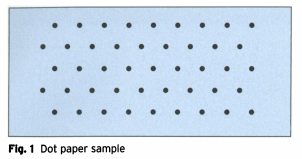
\includegraphics[width=0.33\textwidth]{sierp_fig_1}
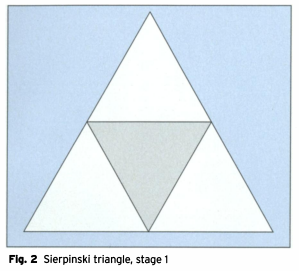
\includegraphics[width=0.33\textwidth]{sierp_fig_2}
\end{center}
To keep overzealous students from merely connecting every dot on the page, students should shade in this newly formed triangle. Next, students connect all the midpoints of the unshaded triangles, forming 3 new triangles, which they should shade in (see fig. 3).
\begin{center}
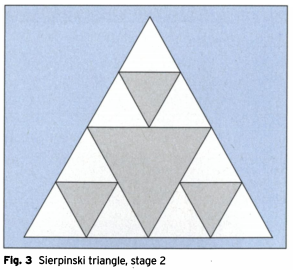
\includegraphics[width=0.33\textwidth]{sierp_fig_3}
\end{center}
This process can be continued indefinitely (although the students lose the benefit of the dots after stage 4, since the starting triangle has sides of length 16), as shown in the following figures:
\begin{center}
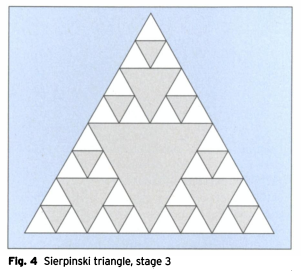
\includegraphics[width=0.33\textwidth]{sierp_fig_4}
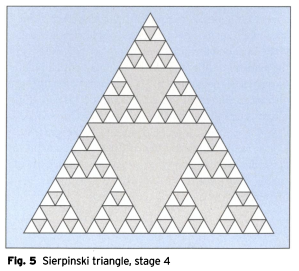
\includegraphics[width=0.33\textwidth]{sierp_fig_5}
\end{center}
%should the illustrations be cited in-line?
Students completing this activity are often surprised at how quickly the number of triangles grows. The growth is exponential, giving the student $3^{(n-1)}$ more triangles to shade at each step. \end{comment}

In an introductory course to ordinary differential equations, a student is introduced to some very simple models which can be useful in science, the most elementary model being 
$$\frac{dx}{dt}=kx,$$
whose solution is 
$$x(t)=e^{kt},$$
that is, exponential growth. 

In actual practice however, models often require quite a bit of "ugliness" to be actually useful. A differential equation may have many parameters, or it may have nonlinear terms such as $\sin$, $\sqrt{\phantom{x}}$, or other parts that make the system difficult to deal with. 

In Strogatz's text, we gained an introduction to some
graphical and intuitive methods for dealing with nonlinear differential equations. This takes much of the "ugliness" and tackles it with pictures, making the problem much more digestible. I eventually was able to read a research paper, applying these biology to biology, exploring a population model that uses a nonlinear term to represent the effect of fear on the population of the prey. 

\subsection{Using Differential Equations}

%A. What is a differential equation? How do you solve one, and what do its solutions mean? Very brief mention of the usual methods of solving them, emphasising that the advantage of the methods of this paper is that they avoid the textbook methods.

We began this course with the assumption that every had already had a full course on differential equations. Here I get our feet wet with a reminder of the basics and a few definitions. A \emph{differential equation} describes a real life system by, instead of giving an equation which represents its location or state, giving an equation for how its state is changing. For example, in the equation 
\begin{equation}
\frac{dx}{dt}=x,
\end{equation}
the change in $x$ as time $t$ changes is equal to the actual value of $x$. That is, as $x$ grows, the rate of growth of $x$ also grows. A \emph{solution} to a differential equation is an explicit function which gives $x$ as a function of $t$, and which satisfies the differential equation. A solution to (1) is shown below, with $x$ on the vertical axis and $t$ on the horizontal axis:
\jpg{width=0.3\textwidth}{exp-x}
Look familiar? This is exponential growth, because the differential equation above can be solved as follows:
\[\begin{array}{rrcll}
&\dfrac{dx}{dt}&=&x\\
&\dfrac{1}{x}dx &=& dt & \text{separate the variables}\\
&\ln(x)&=&t+C& \text{integrate both sides}\\
\phantom{\text{exponentiate both sides}}&x&=&e^t e^C& \text{exponentiate both sides}\\
&x&=&x_0 e^t& \text{explanation below}\\
\end{array}\]
It turns out that $e^C$ is the initial value of $x$, so we notate it $x_0$ (to see this, try plugging in $t=0$). This process above is fairly straightforward if you're comfortable with calculus, but can you imagine trying to solve something like 
$$\dfrac{dx}{dt}=x\left[r-a(x-b)^2\right]$$
using a similar method? \footnote{This is one formulation of the Alee effect. In this equation, $a,b,$ and $r$ are constants. See Strogatz section 2.3 for more.} Suffice it to say, symbolic methods are important, but not always an effective way to solve real-life differential equations. 

\subsection{A Geometric Way of Thinking}

%B. Introduction to Strogatz’s method of exploring the basic qualities of a nonlinear system by graphing, and aided by elementary calculus. 

In his book, \textit{Nonlinear Dynamics and Chaos}, Steven Strogatz gives a brilliantly intuitive way of dealing with with differential equations, using pictures. Consider the following example:
\begin{equation}
\dot{x}=\sin x.
\end{equation}
(By the way, we will simplify the notation from now on by writing $\dot{x}$ to mean $\frac{dx}{dt}$.) This equation is solvable using the symbolic strategy we used for (1), although many nonlinear systems are impossible to solve in closed-form. However, the solution would fit many people's definition of "ugly":
\begin{equation}
t=\ln\left|\frac{\csc x_0 + \cot x_0}{\csc x + \cot x}\right|.
\end{equation}
While correct, this result is in many ways unhelpful. For example, what does $x(t)$ do as $t\to\infty$? This is a basic question we might ask about any system, and it is difficult to say without a computer-generated plot.

Instead, let us take a graphical approach. The funtion $\sin x$ is very easy to graph, and graphing $\dot{x}$ versus $x$ reveals a lot of information about the system. If we think of $x$ as the position of an imaginary particle on the horizontal axis, then $\dot{x}$ tells us the velocity of that particle. 
\jpg{width=0.75\textwidth}{stro_fig_2-1-1}
On the figure here (Figure 2.1.1 in Strogatz), the arrows show that when $\dot{x}$ is positive, $x$ is moving to the right; and when $\dot{x}$ is negative, $x$ is moving to the left. This allows us to very easily answer our question from earlier- what happens as $t\to\infty$? By following the arrows, you can see that given any starting point, $x$ will move away from a hollow point and towards a solid point. At those points, $\dot{x}=0$, which means that $x$ doesn't move. These points are called \emph{fixed points}. As you can see, there are two kinds of fixed points. The solid dots in the picture represent \emph{stable} fixed points, because any point nearby will "settle in" towards such a fixed point. The hollow dots are called \emph{unstable} fixed points, because while starting exactly on an unstable fixed point will result in no movement, even a tiny perturbation to one side or the other will cause the state of the system, or the \emph{phase}, to move away from the unstable fixed point. 

You may notice that the picture is sloping upward at all the unstable fixed points, and downward at the stable ones. This means that we can obtain quite a lot of information about a system using just a bit of calculus. If your system is 
$$\dot{x}=f(x),$$
then all the fixed points can be found by solving $f(x)=0$, and one can determine their stability using the derivative:
\[\text{A fixed point } x^* \text{ is} \quad
\begin{cases}
\text{stable} & \text{if } f'(x^*)<0\\
\text{unstable} & \text{if } f'(x^*)>0\\
\end{cases}
\]

\subsection{Getting a Model "Dialed-In"}

%C. Definition of stable and unstable fixed points, also definition and illustration of a bifurcation using graphs of a quadratic equation, as in Edwards’ paper (with help from Desmos, and section 3.1 in Strogatz). 

Now that we've covered the basics of analyzing these sorts of problems, let's talk about creating a differential equation to use as a biological model. In order for our model to accurately represent the real-life situation, we'll need to involve accurate numbers. To do this, we use parameters. A parameter is a number that is constant within a specific system, but may chance between different applications. For example, a thrown ball and a catapult projectile can both be modeled with parabolas, but the two will require dramatically different numbers. This concept applies to differential equations as well. As an illustration, let's consider the differential equation
\begin{equation}
\dot{x}=ax^2+bx+c.
\end{equation}

Edwards outlines a fantastic method to explore the question "What happens to the graph as we change $a, b$, and $c$?" Edwards suggests using technology to vary the three parameters using sliders, and although he uses an old TI computer algebra system, we will demonstrate his method using Desmos. 

\noindent First, we input the equation, and assign a slider to each parameter. 
\jpg{width=0.5\textwidth}{desmos_1}
The reader is probably already familiar with the effects of changing the $a$ and $c$ parameters, as they are often used in graphing parabolas by hand. Varying $a$ stretches the graph, and changing $c$ causes a vertical shift. Notice how the vertex follows the dotted line as $c$ is changed. 
\begin{center}
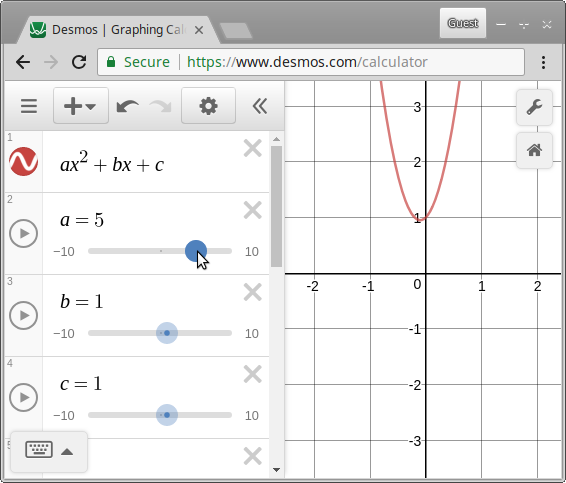
\includegraphics[width=0.45\textwidth]{desmos_2}
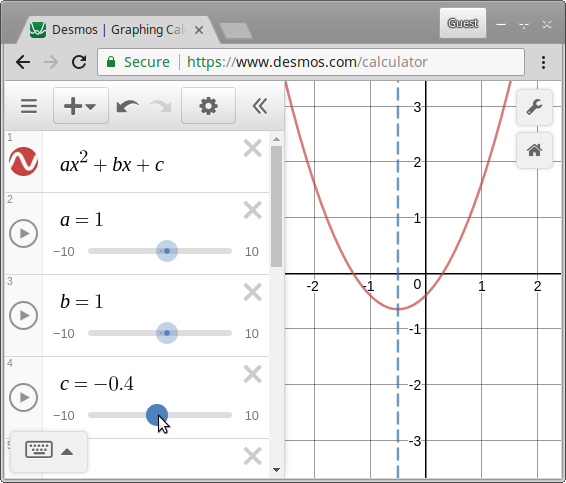
\includegraphics[width=0.45\textwidth]{desmos_3}
\end{center}
What happens when we vary $c$? If you try it, you'll see that the graph shifts around, but not in a linear way. You may not see it at first, but amazingly, the vertex actually traces out an inverted parabola! Try this at home, starting out with different $a$ and $c$ values, to see how the vertex always traces out a parabola as $b$ is varied. 
\begin{center}
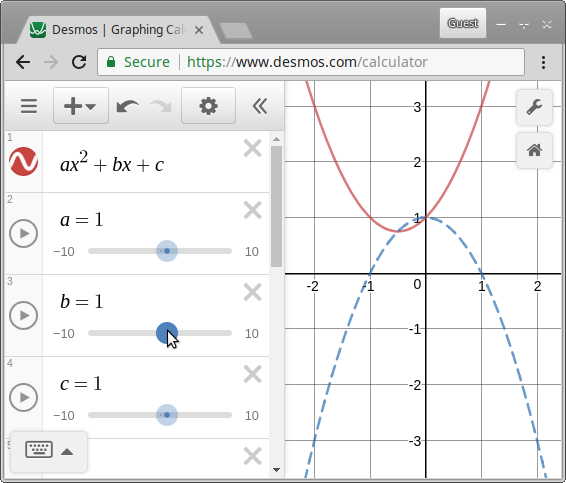
\includegraphics[width=0.3\textwidth]{desmos_4}
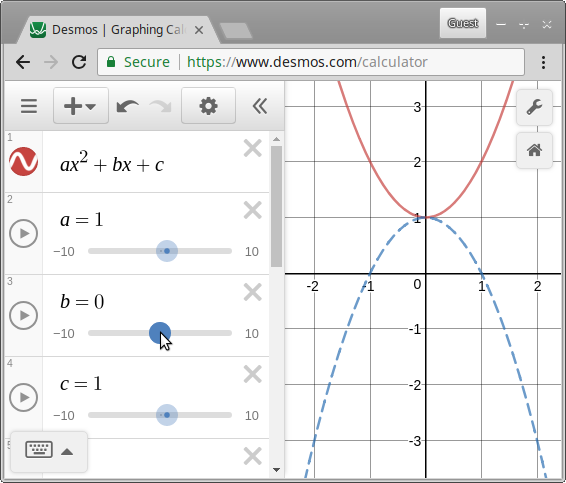
\includegraphics[width=0.3\textwidth]{desmos_5}
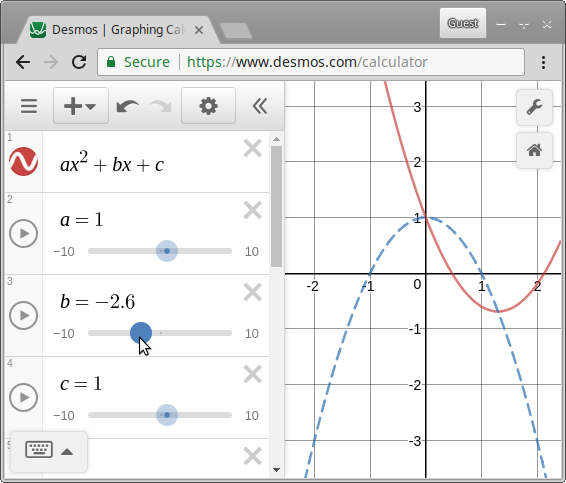
\includegraphics[width=0.3\textwidth]{desmos_6}
\end{center}
You may be asking yourself, "How does this relate to differential equations?" Well, when we interpret this parabola as a graph of $\dot{x}$ versus $x$, we'll see that something very interesting happens with the stable points when one or more of those parameters are changed. Consider this phase portrait of $\dot{x}=x^2-1$, from the Strogatz text. 
\jpg{width=0.5\textwidth}{stro_fig_2-2-2}
You can see that it has two fixed points, one stable and one unstable. What if we thought of this as a specific case of $\dot{x}=r+x^2$, where $r=-1$? What happens when we vary the parameter $r$?
\jpg{width=0.95\textwidth}{stro_fig_3-1-1}
As you can see, when r is increased enough, the two fixed points merge into one, and then seem to annihilate each other. This is called a \emph{saddle-node bifurcation}, and it is a very important type of bifurcation. Imagine if, for example, a population had a stable fixed point, and a change in a parameter caused the fixed point to disappear? The population would either increase or decrease until it settled into another fixed point, which would have major biological implications. 

\subsection{The Logistic Model}

%D. Introduction to the Logistic Model, as per Brauer. This model can be much more easily analyzed via the graphical methods of Strogatz.

Now that we have all the tools we will need to apply this idea to science, let's explore an actual model. In this section, we will follow the exposition given in the textbook \textit{Mathematical models in population biology and epidemiology}, by Brauer. To establish our notation, $x(t)$ denotes the size of the population at time $t$, and $\dot{x}$ the rate of change of the population with respect to time. At this point, we assume that the population growth rate depends on its size (more organisms will reproduce faster, as in the dice rolling example from earlier) and nothing else. This is a pretty reasonable assumption if we're talking about microorganisms like bacteria, but it would be too simple for anything more complicated like plants, animals, or people. To fully account for all of the different factors which may speed or slow population growth in more complex species, a model might need to account for competition within the species (overpopulation should reduce growth), or age structure (what if the death rate only depends on the number of old organisms, and young ones can be neglected?). It could also be the case that the population growth depends heavily on the population of another species as well as its own if there is competition or predation (or both) going on. 

Since the only variable we're only considering is $x$, our population, how can we model it? We've already thought in depth about the simplest type of model $\dot{x}=Cx$, where the growth rate is assumed to be a constant multiple of the population. In other words, the \emph{growth rate per capita} $\dot{x}(t)/{x}(t)$ is constant. Of course, if we're interested in modeling real-life populations, not even bacteria can grow exponentially for very long. There should be some point at which the population can't grow any more, either because there is no more room in the petri dish, or they have eaten all the food, or for some other reason. The simplest way to model this is to assume that the per capita growth rate starts out at some quantity $\lambda$, and then decreases as the population grows. This gives the famous \emph{logistic equation} 
\begin{equation}
\dot{x}=x(\lambda-ax).
\end{equation}
We can also rearrange this, to represent the maximum population. If $x$ is close to $0$, then the growth rate with be the largest, and then it will steadily decrease until the population reaches a certain amount. This alternate formulation is written 
\begin{equation}
\dot{x}=rx\left(1-\frac{x}{k}\right),
\end{equation}
Where $r=\lambda$ and $k=\lambda/a$. As you can see, when $x\approx0$, the second factor equals 1, and the population grows exponentially. But, as the population increases so that $x=k$, the second factor vanishes, and so does $\dot{x}$. $r$ is called the \emph{intrinsic growth rate}, and $k$ is called the \emph{carrying capacity}. The logistic equation is solvable symbolically (though it requires quite some effort). A few solutions are shown below, to give the reader a visual idea of how the system behaves. 
\jpg{width=0.5\textwidth}{brauer_fig_1-1}
Could we have analyzed this system in some other way? Of course, let's use the graphical method of Strogatz. To get a better look, distribute the $x$ in equation (5). 
$$\dot{x} =-ax^2+\lambda x$$
Now we see that this is a parabola, with which we are well acquainted. In fact, we can even determine the location and stability of the fixed points in (5) without graphing. As we have previously mentioned, there is a fixed point $x^*$ wherever $\dot{x}=0$, so our fixed points lie at 
$x^*=0$
and 
$(\lambda-ax^*)=0$
or $x^*=\lambda/a$. To check the stability of these points, we only need determine if $f'(x^*)$ is positive or negative at each point. Since $f(x)=-ax^2+\lambda x$, $f'(x)=-2ax+\lambda$, then $f'(0)>0a$ as long as $\lambda>0$ (this has to be true, otherwise equation (5) doesn't make much sense), so $0$ is unstable. Also, $f'(\lambda/a)=-\lambda$, so this fixed point is stable for the same reason. 

The interpretation of all this is that, regardless of the specific values of the parameters $a$ and $\lambda$, we will always see a stable fixed point, representing the carrying capacity, and an unstable fixed point at $x=0$. 

\subsection{A (Slightly) More Complex Model}

%E. Slight modification of the logistic model, adding a predation/fear parameter, in the style of the paper by Wang (although here we use a simplified version).

As we mentioned earlier, the logistic model does a great job for modeling population growth of very simple organisms, but should be augmented to model more complex organisms. In their paper "Modelling the fear effect in predator-prey
interactions", the authors explore just such a model. They start with three different parts:
$$\dot{x}=rx-dx-ax^2,$$
Where $r$ is the species' birth rate, $d$ is its
natural death rate, and $ax$ gives the death rate due to intra-species competition (notice how this last term has an $x$ in it; $a$ is really the parameter here, but it should makes sense to think of $-ax$ getting more negative as the population increases). Wang et al proceed to consider the population $y$ of predators in their model, including a predation term $-py$, but we will omit it for simplicity.

In the field, recent experiments have shown that predators can affect the population of prey in ways other than directly preying on them. For example, the prey could respond to its fear of predators by changing its habitat usage, foraging behavior, and sleep patterns. %more could be added here if necessary
To account for this, Wang et al added a predation term $f(k,y)$ which gives the effect on birth rates as a function of fear level $k$ and predator population $y$. To simplify the analysis, we will consider $f$ to be a parameter, and observe how it changes the dynamics. Thus, our latest model is given by 
$$\dot{x}=rx-dx-ax^2-f.$$

\subsection{Analyzing the Model}

%F. Through our graphical methods, we see that a bifurcation can happen as the rate of predation changes. If the predation rate grows too large, the stable fixed point disappears, and the population rate is negative everywhere, leading to extinction.

We can can rearrange the model above to simplify things. It is essentially a quadratic equation of the form 
$$\dot{x}=-ax^2+(r-d)x-f.$$
As we increase $f$ to represent stronger effect of fear, we see the same sort of situation we've seen before; a bifurcation. Increasing the value of $f$ causes a vertical shift in the graph. Observe what happens to the fixed points:
\begin{center}
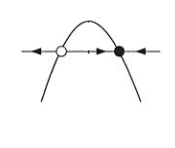
\includegraphics[width=0.3\textwidth]{stro_fig_3-1-1_rev_a}
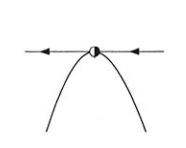
\includegraphics[width=0.3\textwidth]{stro_fig_3-1-1_rev_b}
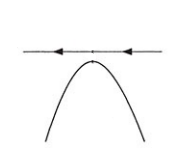
\includegraphics[width=0.3\textwidth]{stro_fig_3-1-1_rev_c}
\end{center}
As the effect of fear becomes stronger past a certain point (that is, when $f>\frac{r-d}{2a}$), the stable fixed point disappears and we see that the population decreases until the species becomes extinct.

\subsection{Conclusion} 
In this semester, we briefly discussed the definition and interpretation of a differential equation, and its usefulness in modeling populations. In our discussion of population models, we found that many functions which are useful modeling are not easy to analyze, but the graphical method of Strogatz gave us a very powerful and  very useful tool to use pictures to learn the qualitative aspects of the model, and an insight into bifurcations and how they work. We also discussed multi-dimensional systems and methods, though those processes are not given in this report. 

\section{What I Learned in Other Students' Lectures}
\subsection{Watching Other Students Teach}
Watching the lectures given by other students has been a beneficial experience for me. I was able to pick up a lot of tips that I can use in my own teaching; learning what \emph{to} do as well as what \emph{not} to do. 

One thing I learned was the importance of standard and consistent letter formation, especially Greek letters. It is important that the audience can understand what I am teaching, and it also takes up valuable class time if I have to answer questions such as "Is that a 'phi' or a 'theta'?". It is also important that I research and know the correct way to say the names of Greek letters, and teach them to my students. I have noticed that there are times when a presenter is unsure about the name or pronunciation of a letter ($\xi$, for example), and the speaker's unsureness about the letter can result in the audience's unsureness about the math. 

I have also learned about the importance of enthusiasm and variation in the tone of one's voice when presenting. Most of my professors over the years have been very good as this, and the effect was greatly exaggerated when this was juxtaposed with watching an inexperienced student present in a completely monotone voice. With this goes an aspect of confidence. I think that this is often improved with practice and coaching, and conscious effort. 

One tip that I picked up this semester is that much can be gained from giving a "practice" presentation to a classmate or colleague. Eli and I often presented to each other a day or two before, and this gave us an opportunity to point out areas of improvement in each others' presentations. 

\subsection{Applying What I Learned}

I felt that my final presentation for Math 493 was one of my all-time best college math presentations. Part of this was my chance to practice presenting with a slide clicker, when I gave my PUMP presentation with Eli early this spring. Another student brought the clicker, and we used it in our presentation, although awkwardly. I liked it so much that I bought one for myself and practiced presenting with it in my empty high-school classroom after work. I think this improved my final presentation, and helped it to feel more "polished". 

I also found that adding just a small amount of humor to a presentation can greatly improve audience engagement and enjoyment. While using formal mathematical language is critical to accurately communicate mathematical ideas, allowing oneself to digress from formal language occasionally can provide the audience with a chance to relax, and can help release tension about a particularly gnarly\footnote{By the way, the Google "define" search widget gives the definition of gnarly as: (1) Gnarled, as in a root or branch. (2) Difficult, dangerous, or challenging; as in "she battled through the gnarly first sequence."} equation or theorem. 

I feel that my presenting ability has grown this semester, and that I am better prepared for college lecturing, as a PhD student and someday as a professor myself. 

\section{My Reading in the Paper}
The paper I read was \emph{Modelling the fear effect in predator–prey interactions}, by authors Xiaoying Wang, Liana Zanette, and Xingfu Zou, published in Mathematical Biology in 2016. Reading this paper was a challenge, and I feel that I experienced growth in the process. One part that was particularly difficult for me was parsing and interpreting the model, because the authors chose not to denote the parameters with the same initial letter as their meanings. For example, birth rate and intra-species competition were denoted $r_0$ and $a$, respectively. In my presentation, I chose to change the notation, using $x$ and $y$ as the variables instead of $u$ and $v$, and also denoted the parameters with their initial letters, i.e. $b$ for birth rate, $c_1$ for competition, $c_2$ for biomass conversion rate.  I think this helped me understand the paper better because I was able to take some personal ownership of the material, having made a small choice to make it more understandable for me. It was also helpful that in order to make those changes in my notes, I had to read the equations very carefully. 
\subsection{Motivation}
In predator-prey dynamics, the longstanding view is that predators only affect prey via predation. However, recent research shows that fear alone can reduce prey reproduction rates.

\mbox{}

Fear can effect:
\begin{itemize}
\item Habitat Usage
\item Foraging behaviors
\item Vigilance
\item Physiological changes
\end{itemize}

In a recent experiment on songbirds, the birds were protected from predation, but had sounds of their predators played nearby for an entire breeding season. It was found that birth rates were reduced by an average of 40\%.

\subsection{Introduction}
%%%%%%%%%%%%%%%%%%%%%%%%%%%%%%%%%%%%%%%%%%%%%%%%%%
%NEED A FRAME ABOUT MOTIVATION AND BACKGROUND
%%%%%%%%%%%%%%%%%%%%%%%%%%%%%%%%%%%%%%%%%%%%%%%%%%


First, we begin with a basic logistic model. 
$$\dot{x}=bx-dx-c_1x^2$$

\begin{center}
\begin{tabular}{rl}
$x$& population of prey\\
$b$& birth rate of prey (natural)\\
$d$& death rate of prey (natural)\\
$c_1$& competition-related death rate of prey\\
\end{tabular} 
\end{center}
Note, all parameters and variables are positive numbers. 
  
%    \begin{columns}
%        \begin{column}{.33\textwidth}
%			
%        \end{column}        
%        \begin{column}{.66\textwidth}
%           
%        \end{column}
%    \end{columns}


%%%%%%%%%%%%%%%%%%%%%%%%%%%%%%%%%%%%%%%%%%%%%%%%%%%%

Next, we multiply by a factor which reduces the birth rate due to fear effects. 
$$\dot{x}=[f(k,y)b]x-dx-c_1x^2$$
Here, $k$ is a parameter which reflects the strength of the fear effect, and $y$ is the population of the predator.


%%%%%%%%%%%%%%%%%%%%%%%%%%%%%%%%%%%%%%%%%%%%%%%%%%%%

$$\dot{x}=[f(k,y)b]x-dx-c_1x^2$$

\mbox{}

So, what sort of a function is $f(k,y)$? We'd like to think of it generally for now, but there are some things we can say for sure about it:

\mbox{}

\begin{highlight}
\begin{tabular}{rl}
$f(0,y)=f(k,0)=1$ & No fear/predators, full birth.\\
\\
$\frac{\del f}{\del k}<0, \frac{\del f}{\del y}<0$& More fear/pred, less birth.\\
\\
$\lim\limits_{y\to\infty}f(k,y)=\lim\limits_{k\to\infty}f(k,y)=0$& Maximum effect is 0 birth.\\
\end{tabular}
\end{highlight}

\mbox{}

In short, $f:\R^+\times\R^+\to[0,1]$ is monotonically decreasing when thought of as a function of either $k$ or $y$. 

%%%%%%%%%%%%%%%%%%%%%%%%%%%%%%%%%%%%%%%%%%%%%%%%%%%%

Next, we'll add in a predation function, $g(x)$, and include the predator population dynamics into our system. 

\[\begin{array}{rcl}
\dot{x}&=&[f(k,y)b]x-dx-c_1x^2-g(x)y\\
\dot{y}&=&[g(x)c_2]y-my
\end{array}\]

Here, $m$ is the mortality rate of predators, and $c_2$ is the conversion rate of prey's biomass to predator's biomass. That is, we are assuming that the predators' birth rate is directly proportional to predation. 


%%%%%%%%%%%%%%%%%%%%%%%%%%%%%%%%%%%%%%%%%%%%%%%%%%%%
%{About $g(x)$}
Typically, the predation $g(x)$ is modeled in one of two ways:

\begin{itemize}
\item In a linear functional response, $$g(x)=px,$$ which assumes that predation is directly proportional to prey population.
\item In a Holling Type II functional response, $$g(x)=\frac{px}{1+qx},$$ which assumes that predation increases quickly as prey population increases, and then tapers off to approach $\frac{p}{q}$ asymptotically. 
\end{itemize}

%%%%%%%%%%%%%%%%%%%%%%%%%%%%%%%%%%%%%%%%%%%%%%%%%%%%
\subsection{Linear Functional Response}

Let's explore the model, assuming a linear functional response for predation. So, $g(x)=px$, where $p$ is a parameter that represents the predation rate. 

\[\begin{array}{rcl}
\dot{x}&=&[f(k,y)b]x-dx-c_1x^2-pxy\\
\dot{y}&=&pc_2xy-my
\end{array}\]

Where are the fixed points? 

%%%%%%%%%%%%%%%%%%%%%%%%%%%%%%%%%%%%%%%%%%%%%%%%%%%%
\subsubsection*{Finding Fixed Points}

%\[\begin{array}{rcl}
%\dot{x}&=&[f(k,y)b]x-dx-c_1x^2-pxy\\
%\dot{y}&=&pc_2xy-my
%\end{array}\]

%\mbox{}

There are (at most) 3 fixed points:
\begin{itemize}
\item $E_0=(0,0)$. This is a fixed point because
\[\arraycolsep=1.4pt\def\arraystretch{1.5}
\begin{array}{rcll}
\dot{x}&=&[f(k,0)b](0)-d(0)-c_1(0)^2-p(0)&=0\\
\dot{y}&=&pc_2(0)-m(0)&=0
\end{array}\]
\end{itemize}

%%%%%%%%%%%%%%%%%%%%%%%%%%%%%%%%%%%%%%%%%%%%%%%%%%%%

%\[\begin{array}{rcl}
%\dot{x}&=&[f(k,y)b]x-dx-c_1x^2-pxy\\
%\dot{y}&=&pc_2xy-my
%\end{array}\]

%\mbox{}

\begin{itemize}
\item $E_1=\left(\frac{(b-d)}{c_1},0\right)$, when $b>d$. To see that this is a fixed point, 
\[\arraycolsep=1.4pt\def\arraystretch{1.5}
\begin{array}{rcll}
\dot{y}&=&pc_2(0)-m(0)\\
&=&0 \\
\dot{x}&=&[f(k,0)b]\left(\frac{(b-d)}{c_1}\right)-d\left(\frac{(b-d)}{c_1}\right)-c_1\left(\frac{(b-d)}{c_1}\right)^2-p(0)\\
&=&\frac{1}{c_1}\left[(1)b(b-d)-d(b-d)-(b-d)^2\right]\\
&=&\frac{1}{c_1}\left[b^2-2bd+d^2-(b-d)^2\right]\\
&=&0.
\end{array}\]
\end{itemize}

%%%%%%%%%%%%%%%%%%%%%%%%%%%%%%%%%%%%%%%%%%%%%%%%%%%%

%\[\begin{array}{rcl}
%\dot{x}&=&[f(k,y)b]x-dx-c_1x^2-pxy\\
%\dot{y}&=&pc_2xy-my
%\end{array}\]

%\mbox{}

\begin{itemize}
\item $E_2$: If  $\frac{(b-d)}{c_1}>\frac{m}{c_2p}$, then $E_2=\left(\frac{m}{c_2p}, y^*\right)$, where $y^*$ satisfies 
$$b\, f(k,y^*)-d-c_1x^*-py^*=0.$$
(This is $\frac{\dot{x}}{x}=0$). To see that such a $y^*$ exists, observe that this is equivalent to
$$\underbrace{b\, f(k,y^*)-py^*}_{\text{decreasing}}=\underbrace{d+c_1x^*}_{\text{increasing}},$$
and the LHS is $b$ at $y=0$, RHS is $d$ at $x=0$, and $b>d$. 
\end{itemize}

%%%%%%%%%%%%%%%%%%%%%%%%%%%%%%%%%%%%%%%%%%%%%%%%%%%%

\begin{itemize}
\item $E_2$ (continued): 

\mbox{}

To see that $E_2$ is a fixed point: 
\[\begin{array}{rcl}
\dot{x}&=&[f(k,y^*)b]x^*-dx^*-c_1(x^*)^2-px^*y^*\\
&=&([b\,f(k,y^*)]-d-c_1x^*-py^*)x^*\\
&=&0\\
\\
\dot{y}&=&pc_2x^*y^*-my^*\\
&=&pc_2\left(\frac{m}{c_2p}\right)y^*-my^*\\
&=&my^*-my^*\\
&=&0
\end{array}\]
\end{itemize}

%%%%%%%%%%%%%%%%%%%%%%%%%%%%%%%%%%%%%%%%%%%%%%%%%%%%
\subsubsection*{Analyzing Stability}
Thus, we have found 3 fixed points (or equilibria), $E_0, E_1,$ and $E_2$.

Let's analyze their stability. 
\begin{highlight}
\begin{theorem*}\mbox{}
\begin{enumerate}
\setcounter{enumi}{-1}
\item $E_0$ is stable if $(b-d)$ is negative, and unstable if positive.
\item $E_1$ is stable if $\frac{(b-d)}{c_1}<\frac{m}{c_2p}$ (i.e. if $E_2$ does not exist) and is unstable if reversed.
\item $E_2$ is stable as long as it exists (when $\frac{(b-d)}{c_1}>\frac{m}{c_2p}$). 
\end{enumerate}
\end{theorem*}
\end{highlight}
%%%%%%%%%%%%%%%%%%%%%%%%%%%%%%%%%%%%%%%%%%%%%%%%%%%%

It should be intuitively obvious that if $(b-d)<0$, then neither prey nor predator can survive. Observe:
\[\begin{array}{rcl}
\dot{x}&=&[f(k,y)b]x-dx-c_1x^2-pxy\\
&=&(f(k,y)b-d)x-c_1x^2-pxy\\
&\leq&(b-d)x-c_1x^2-pxy\\
&<&0\\
\\
\dot{y}&=&pc_2xy-my\\
&\to&0
\end{array}\]

Thus, $E_0$ is stable if $(b-d)<0$. 

The author omits the proof for stability of $E_1$, because the proof for $E_2$ is similar:

%%%%%%%%%%%%%%%%%%%%%%%%%%%%%%%%%%%%%%%%%%%%%%%%%%%%

\textbf{Claim:} $E_2$ is stable. Recall that $E_2$ exists if  $\frac{(b-d)}{c_1}>\frac{m}{c_2p}$, and $E_2=\left(\frac{m}{c_2p}, y^*\right)$, where $y^*$ satisfies 
$$[f(k,y^*)b]-d-c_1x^*-py^*=0.$$
\begin{proof}
We use the Jacobian:
\[
\arraycolsep=1.4pt\def\arraystretch{1.5}
\begin{array}{rcl}
	\left.\left[\arraycolsep=1.4pt\def\arraystretch{1.5}
	\begin{array}{cc}
		\frac{\del \dot{x}}{\del x} & \frac{\del \dot{x}}{\del y}\\
		\frac{\del \dot{y}}{\del x} & \frac{\del \dot{y}}{\del y}\\
	\end{array}\right]\right|_{\scalebox{.5}{$(x^*,y^*)$}}
	&=&
	\left[\arraycolsep=1.4pt\def\arraystretch{1.5}
	\begin{array}{cc}
		[f(k,y^*)b]-d-2c_1x^*-py^* & \quad bx^*\frac{\del f}{\del y}-px^*\\
		pc_2y^* & \quad pc_2x^*-m\\
	\end{array}\right]
	\\
	%
	&=&	
	\left[\arraycolsep=1.4pt\def\arraystretch{1.2}
	\begin{array}{cc}
		-c_1x^* &  \quad bx^*\frac{\del f}{\del y}-px^*\\
		pc_2y^* & \quad m-m\\
	\end{array}\right]
	=
	\left[\arraycolsep=1.4pt\def\arraystretch{1.2}
	\begin{array}{cc}
		- & \,\,-\\
		+ & \,\,0\\
	\end{array}\right]		
\end{array}	
\]
So since det $>0$ and trace $<0$, $E_2$ is stable. 
%\dot{x}&=&[f(k,y)b]x-dx-c_1x^2-pxy\\
%\dot{y}&=&pc_2xy-my
\end{proof}

%%%%%%%%%%%%%%%%%%%%%%%%%%%%%%%%%%%%%%%%%%%%%%%%%%%%
\subsection{Holling Type II Functional Response}
Now we've explored the dynamics assuming that the predation function $g(x)$ is a linear function, but it should agree with your intuition that in nature, predation levels with be roughly the same if the prey population is above a certain level. So in this section, we explore the dynamics when $g(x)$ is the following:
%\begin{columns}
%	\begin{column}{0.33\textwidth}
%		$$g(x)=\frac{px}{1+qx}.$$
%	\end{column}
%	\begin{column}{0.66\textwidth}
%		\jpg{width=\textwidth}{holling_type_ii}
%	\end{column}
%\end{columns}
\jpg{width=.618\textwidth}{holling_type_ii}

%%%%%%%%%%%%%%%%%%%%%%%%%%%%%%%%%%%%%%%%%%%%%%%%%%%%

We also choose a particular form for $f(k,y)$, namely 
%\begin{columns}
%	\begin{column}{0.33\textwidth}
%		$$f(k,y)=\frac{1}{1+ky}.$$
%	\end{column}
%	\begin{column}{0.66\textwidth}
%		\jpg{width=\textwidth}{f_k_y}
%	\end{column}
%\end{columns}
\jpg{width=.618\textwidth}{f_k_y}
Note that $f$ still has the same general properties we've assumed so far. 

%%%%%%%%%%%%%%%%%%%%%%%%%%%%%%%%%%%%%%%%%%%%%%%%%%%%

So our model now takes this form:
\[\arraycolsep=1.4pt\def\arraystretch{2}
\begin{array}{rcl}
\dot{x}&=&\dfrac{bx}{1+ky}-dx-c_1x^2-\dfrac{pxy}{1+qx}\\
\dot{y}&=&\dfrac{pc_2xy}{1+qx}-my
\end{array}\]
Next, we find the fixed points. 

%%%%%%%%%%%%%%%%%%%%%%%%%%%%%%%%%%%%%%%%%%%%%%%%%%%%
\subsubsection*{Analyzing fixed points}

There are two fixed points which are the same as we saw with the linear functional response:
\begin{itemize}
\item $E_0 = (0,0),$
\item $E_1 = \left(\frac{b-d}{c_1}, 0\right)$ if $(b-d)>0.$
\end{itemize}
The following can be confirmed as before using linearization: 
\begin{itemize}
\item $E_0$ is unstable if $E_1$ exists. 
\item $E_1$ is stable if $(b-d)(c_2p-mq)<c_1m,$
\item $E_1$ is unstable if $(b-d)(c_2p-mq)>c_1m.$
\end{itemize}

%%%%%%%%%%%%%%%%%%%%%%%%%%%%%%%%%%%%%%%%%%%%%%%%%%%%

If $E_1$ is unstable, it turns out that there is another fixed point, $E_2$. The authors do not state its coordinates in closed-form, only that it exists when $E_1$ is unstable, and the give the following condition upon which $E_2$ is stable:
\[\left\lbrace\begin{array}{rcl}
b&>&d+\dfrac{c_1(c_2p+mq)}{q(c_2p-mq)}\\
k&>&\dfrac{q(c_2p-mq)^2((b-d)q(c_2p-mq)-a(c_2p+mq))}{c_2^2pc_1(qd(c_2p-mq)+c_1(c_2p+mq))}\\
\end{array}\right.\]
\begin{center}
 Gnarly. 
\end{center}
The point here is that to maintain nonzero prey population, $b>d$. To maintain a stable predator population as well, the birth rate $b$ needs to be high enough above the death rate $d$. In addition, the level of fear $k$ must be above a certain amount as well.

%%%%%%%%%%%%%%%%%%%%%%%%%%%%%%%%%%%%%%%%%%%%%%%%%%%%
\subsubsection*{Hopf Bifurcation}
It turns out that under the right condition\footnote{That condition is $y^*<\frac{a_2-2a_5}{a_4+2a_5}$, where $a_2=\frac{(b-d)q-c_1}{c_2p-mq}, a_4=\frac{dq+c_1}{c_2p-mq}, a_5=\frac{c_1mq}{(c_2p-mq)^2}$.}, $E_2$ is unstable and a stable limit cycle appears. Numerical exploration shows that this only happens if $b$ is high enough above $d$. 
\jpg{width=0.66\textwidth}{hopf_graph_1}

%%%%%%%%%%%%%%%%%%%%%%%%%%%%%%%%%%%%%%%%%%%%%%%%%%%%
\subsection{Conclusion}
So we can see that when accounting for the cost of fear, assuming that the fear function is linear basically results in an effect which is the same as lowering the birth rate of the prey. But, if the parameters are right, the system can bifurcate, and where there was once a stable equilibrium between populations of prey and predator, now there exist oscillations. They can be supercritical or subcritical Hopf bifurcations as well, causing the population to either stabilize, or oscillate wildly until one of species is driven extinct. 

\end{document}

